\chapter{Majority arbiter PUFs}
\label{cap:majorityarbiter}

Most of the attacks described in Sec. \ref{sec:attacksonxorarbiter} increase exponentially in their complexity for a growing number of used \apufs in a \xpuf. 
Hence it can be claimed that arbitrary large \xpufs would constitute a secure \puf in terms of non-invasive modeling attacks.
This is possible because only linear enlargement of \xpufs will lead to exponential growth in time consumption for a successful attack.
To overcome the stability problem of \xpufs mentioned in Sec. \ref{sec:xorarbiterpufs} which currently deter them from been enlarged unlimited the concept of \ac{MV} has been introduced. %\cite{Majzoobi2010FPGALines}.
In terms of completeness it has to be mentioned that \ac{MV} can also be used by the attacker as technique to obtain error less responses of a \puf if needed \cite{Ganji2016PACPUFs} \cite{Ozturk2008TowardsDevices}.

\section{Majority based arbiter PUFs}
\label{sec:majorityarbiter}

To apply \ac{MV} to an \apuf a challenge is evaluated $\gls{m}$ times.
After that the most occurring response is the final response for that challenge.
The combination of \ac{MV} and \apuf is called \mpuf.
In this way the total number of unstable challenges as explained in Sec. \ref{sec:arbiter} get reduced and the robustness of the \apuf increases.
Every challenge has a different stability which is the likelihood to not flip its response.
These values vary between $50 \%$ and $100 \%$.
The closer the value is to $50 \%$ the more \acp{MV} are necessary to get a more precise response for this challenge.
Hence how many votes are needed depends on the robustness of the \apuf that is required. 
For a more exact view on the relations between robustness and the number of votes different combinations will be simulated and evaluated in Chap. \ref{cap:stabilitysimulation}.

%========================================

\section{Majority based XOR arbiter PUFs}
\label{sec:majorityxorarbiter}

To make \xpuf secure against modeling attacks they have to use a large amount of \apufs which involves an decrease in their stability.
To boost the stability of \xpufs \ac{MV} is used for every single \apuf instead of the complete \xpuf as shown in Fig. \ref{fig:majorityxorarbiter}.
The stability of the \xpuf increases with the increase of the stability of every \mpuf.
As the stability decreases with higher $\gls{k}$ this has to be counteracted with an larger amount $\gls{m}$ of \acp{MV}.
How these competing values relate and how the stability values of the challenges for large \mxpufs are distributed will be examined in Chap. \ref{cap:stabilitysimulation}.

\begin{figure}[ht]
\centering
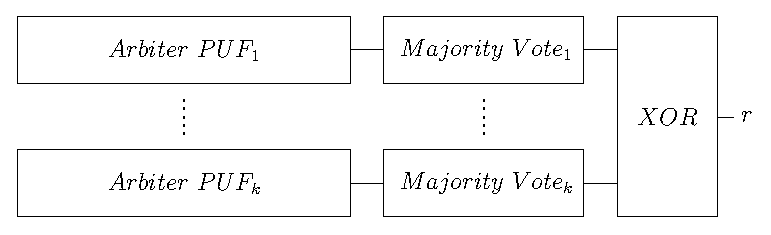
\includegraphics[width=1.00\textwidth]{images/majority_xor_arbiter.eps}
% \noindent\includegraphics[width=1.00\textwidth, height=3cm, draft]{example-image-a}
\caption{\mxpuf}
\label{fig:majorityxorarbiter}
\end{figure}

%========================================

\section{Combiner functions}
\label{sec:combinerfunctions}
% \section{Majority based bent arbiter PUFs}
% \label{sec:majoritybentarbiter}

Beside the \ac{XOR} function other Boolean functions could be used to combine multiple \apuf.
Additionally to being a Boolean function it is important that the function obfuscates the single responses of the \apufs otherwise they can be directly vulnerable to modeling attacks on \apufs.
Bent functions are a type of Boolean function which meets these requirements for example. % [https://en.wikipedia.org/wiki/Avalanche_effect#Strict_avalanche_criterion]
They are highly non-linear which is desired in this case as the \apuf itself is linear and can therefore badly resist machine learning attacks.
Beyond that Bent functions fulfill the strict avalanche criterion.
The strict avalanche criterion means if a single input bit is flipped every output bit flips with a likelihood of $50 \%$.
This prevents predictions about the input based on an analysis of the output of the function.
In this work I focus only on the \ac{XOR} function as combiner function and will not further investigate other possible combiner functions.

%========================================
% source?!
